
\section{Resultados}

\subsection{Red de interacciones y robustez}

La siguiente imagen muestra la red de interaciones del ser humano con las proteínas del SARS-CoV. Como podemos ver el SARS-CoV interacciona con 89 proteínas humanas, produciendo un total de 475 interacciones. 
\begin{figure}
	\centering
		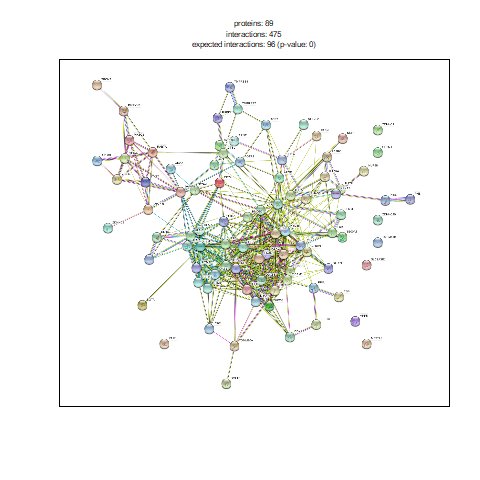
\includegraphics[width=70mm,scale=1.2]{figures/string_hits.png}
		\caption{\textit{Red de interacciones del SARS-CoV con las proteínas humanas}}
\end{figure}

Tras eliminar los nodos que no están conectados, hemos obtenido la red real de interacciones que podemos ver a continuación. Sin embargo hay demasiadas conexiones como para poder distinguir los nodos. Es por ello que realizaremos los pasos siguientes de clustering, para así poder extraer la información relevante de la red. 
\begin{figure}
	\centering
		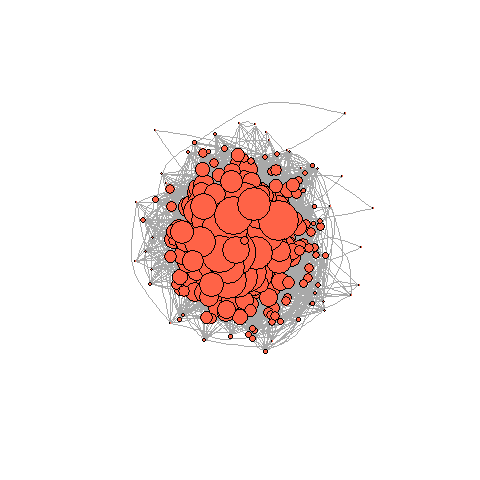
\includegraphics[width=70mm,scale=1.2]{figures/hits.network_graph.png}
		\caption{\textit{Red de interacciones del SARS-CoV con las proteínas humanas tras un proceso de filtrado}}

\end{figure}

Para poder estudiar cual es la capacidad de nuestra red de mantener sus funciones frente a la presencia de "ataques" y ver cuán de adaptable es, usamos la robustez. Podemos observar que para ataques aleatorios es bastante robusta, mientras que para ataques dirigidos es más débil. 
\begin{figure}
	\centering
		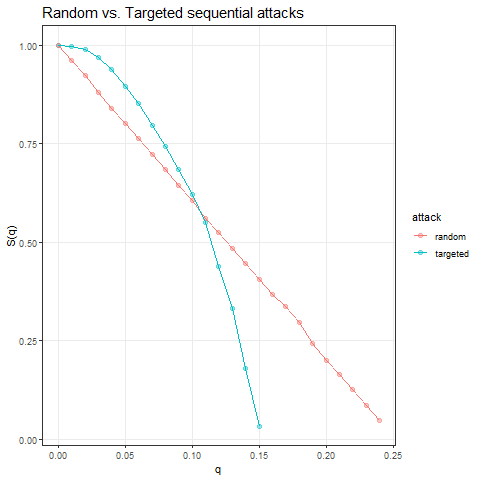
\includegraphics[width=70mm,scale=1.2]{figures/sequential_attacks.png}
		\caption{\textit{Robustez frente a ataques dirigidos y aleatorios}}
\end{figure}

\subsection{Linked Communities}
En esta sección se explicarán los resultados obtenidos aplicar los métodos de comunidades enlazadas a nuestra red, para los cuales hemos usado el paquete linkcomm.

Para ello, primero hemos obtenido estas comunidades aplicando un 'single clustering'. Se ha guardado una imagen del resumen de estas comunidades para un resultado más visual.

 \begin{figure}
 	\centering
 	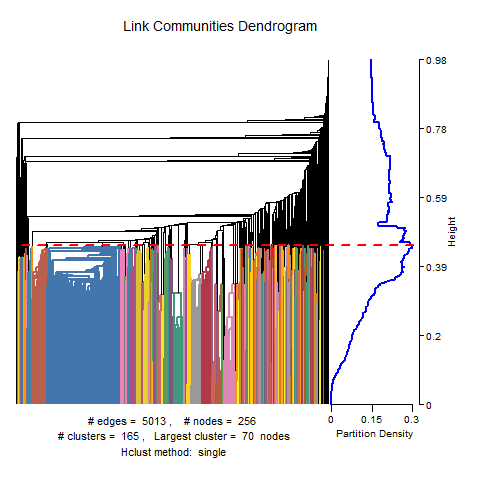
\includegraphics[width=70mm,scale=1.2]{figures/covid_lc_summary.png}
 	\caption{\textit{Esquema de las comunidades obtenidas}}
 \end{figure}

Podemos observar que este método ha definido 165 comunidades diferentes, la mayor de estas tiene 70 nodos lo cual podemos deducir que hay varias comunidades que comparten nodos.

Para poder analizar un poco las comunidades las hemos filtrado por tamaño y modularidad. Las gráficas generadas para este propósito las mostramos a continuación.

 \begin{figure}
	\centering
	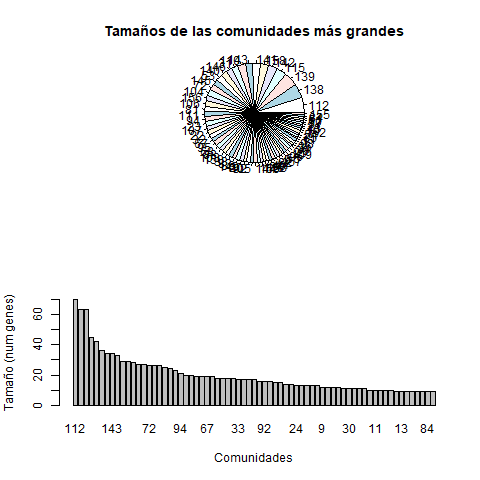
\includegraphics[width=70mm,scale=1.2]{figures/lc_larger_clusters.png}
	\caption{\textit{Comunidades por tamaño}}
\end{figure}

 \begin{figure}
	\centering
	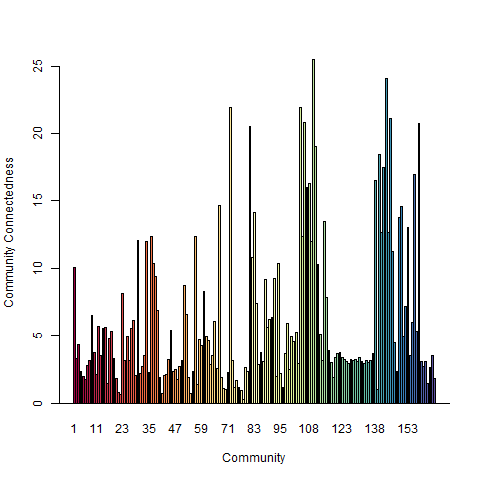
\includegraphics[width=70mm,scale=1.2]{figures/clusters_modularity.png}
	\caption{\textit{Comunidades por modularidad}}
\end{figure}

De estas gráficas hemos podido extraer la comunidad 112 siendo esta la más grande y las comunidades 78 y 22 con una mayor modularidad. Estas comunidades serán utilizadas posteriormente para un análisis funcional.

Para una mejor visualización de los resultados, se ha cambiado el diseño de la gráfica al de Fruchterman Reingold, mostrando solo nodos que pertenezcan a 10 o más comunidades.

\begin{figure}
	\centering
	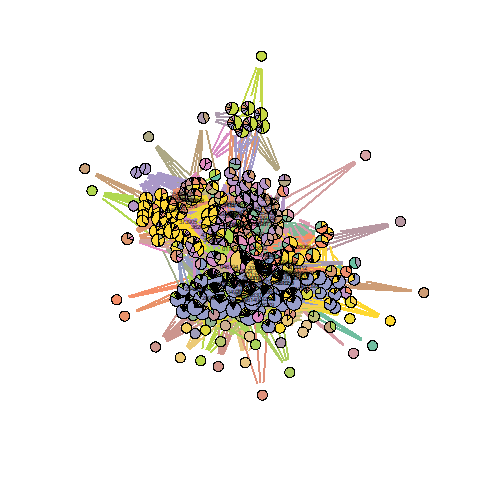
\includegraphics[width=70mm,scale=1.2]{figures/hits.network_layout_fruchterman.reingold_shownodesin_10.png}
	\caption{\textit{Fruchterman Reingold graph}}
\end{figure}

Por otra parte, se han obtenido las comunidades anidadas y se han filtrado para que se muestren las que son independientes de las demás.

 \begin{figure}
 	\centering
 	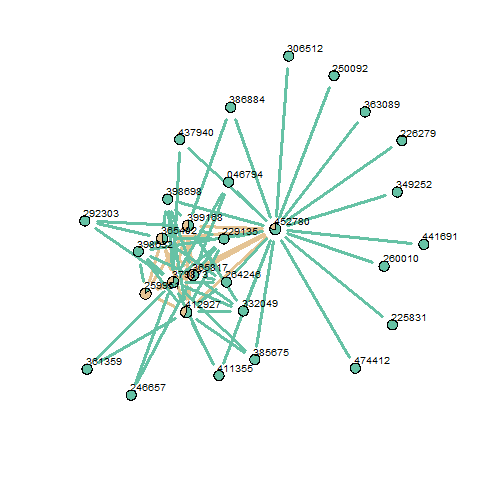
\includegraphics[width=70mm,scale=1.2]{figures/nested_comm.png}
 	\caption{\textit{Comunidades anidadas}}
 \end{figure}